\documentclass[twocolumn, 11pt]{article}%
\usepackage{amsmath, amssymb, esint, gensymb}
\usepackage{graphicx, cuted, geometry, float, chemfig}

\geometry{
    a4paper,
    total={170mm,260mm},
}

\begin{document}

\begin{strip}
  \vspace*{\dimexpr-\stripsep}
  \begin{center}
      \Large\textbf{FISIKA 2}\\
      \large{Pertemuan 1 - Minggu 2 (443483)}\\
      \large{\today}
   \end{center}
\end{strip}

\section{Medan Listrik Oleh Muatan Terdistribusi Kontinu}
    \subsection{Konsep Awal}
    Dari sini akan dibahas medan listrik oleh muatan terdistribusi kontinu yang homogen, atau persebarannya merata. Medan listrik yang ditimbulkan oleh elemen muatan $\Delta q$ adalah:
    \[ \Delta \vec E = k \frac{\Delta q}{r^2} \hat r \]

    Perlu diingat bahwa
    \[k = \frac1{4\pi \epsilon_0}\]

    Medan listrik karena gabungan "elemen" muatan adalah:
    \[ \Delta \vec E = \sum_i \Delta \vec E_i = k \sum_i \frac{\Delta q_i}{r_i^2} \hat r_i \]
    
    Dimana $\hat r$ dan $\hat r_i$ adalah vektor satuan $\Delta q$ untuk menghitung arah dari $\Delta \vec E$. Jika $\Delta q \rightarrow dq \rightarrow 0$, penjumlahannya berubah menjadi integral.\\

    \subsubsection{Bidang Satu Dimensi (batang)}%
    Jika muatan didistribusikan di sepanjang segmen garis lurus yang sejajar dengan sumbu $x$, besarnya muatan $dQ$ pada segmen dengan panjang $dx$ adalah $\lambda dx$
    \begin{center}
        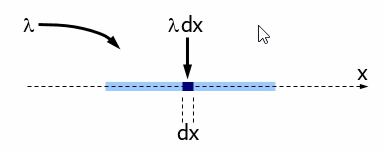
\includegraphics[width=200px]{1.png}
    \end{center}

    $\lambda$ adalah massa jenis muatan (jumlah muatan per satuan panjang). $\lambda$ bisa juga menjadi fungsi posisi.

    Jika $\lambda \iff \ell \iff$ panjang, maka $\lambda$ dikali panjang ruas garis adalah total muatan pada ruas garis.

    \begin{center}
        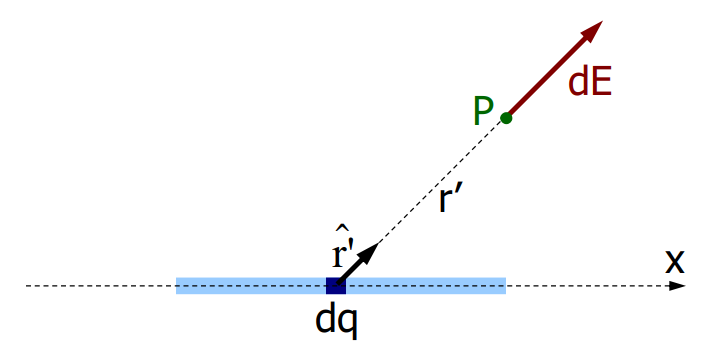
\includegraphics[width=210px]{2.png}
    \end{center}

    Medan listrik di titik P karena muatan $dq$ adalah
    \[d\vec E=k \frac{dq}{r'^2} \hat r = k \frac{\lambda dx}{r'^2} \hat{r'} \]

    \begin{center}
        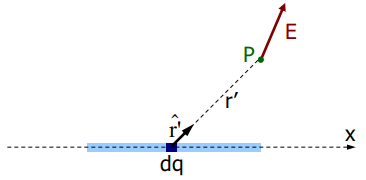
\includegraphics[width=210px]{3.png}
    \end{center}
    
    Medan Listrik di titik P karena seluruh garis muatan adalah
    \[\vec E=k \int \hat{r'} \frac{\lambda(x) dx}{r'^2} \]

    Integrasi dilakukan di seluruh panjang garis yang tidak harus tegak lurus. Juga, $\lambda$ bisa menjadi fungsi posisi, dan dapat diambil di luar integral \textbf{ hanya jika distribusi muatan seragam.}

    \subsubsection{Bidang Dua Dimensi}%
    Jika muatan didistribusikan pada permukaan dua dimensi, jumlah muatan $dq$ pada bagian permukaan yang sangat kecil adalah $\sigma\ dS$, dimana $\sigma$ adalah massa jenis muatan (jumlah muatan per satuan luas).

    \begin{center}
        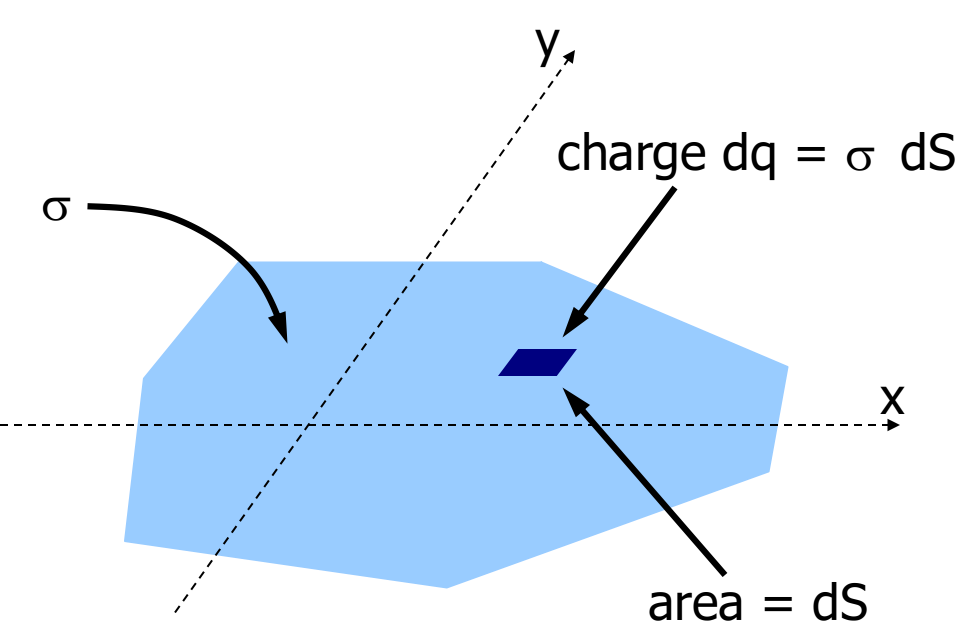
\includegraphics[width=200px]{4.png} 
    \end{center}

    Lalu Medan listrik pada titik P karena seluruh permukaan muatan adalah..
    \[\vec E=k\int\limits_s \hat{r'} \frac{\sigma(x,y) dS}{r'^2} \]
    \begin{center}
        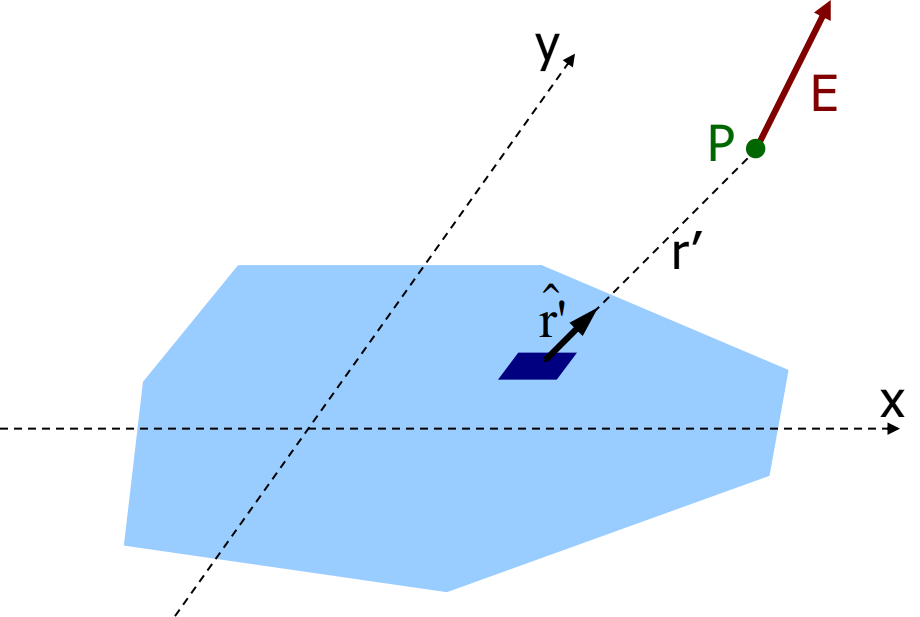
\includegraphics[width=200px]{5.png}
    \end{center}

    \subsubsection{Bangun 3 Dimensi}%
    \begin{center}
        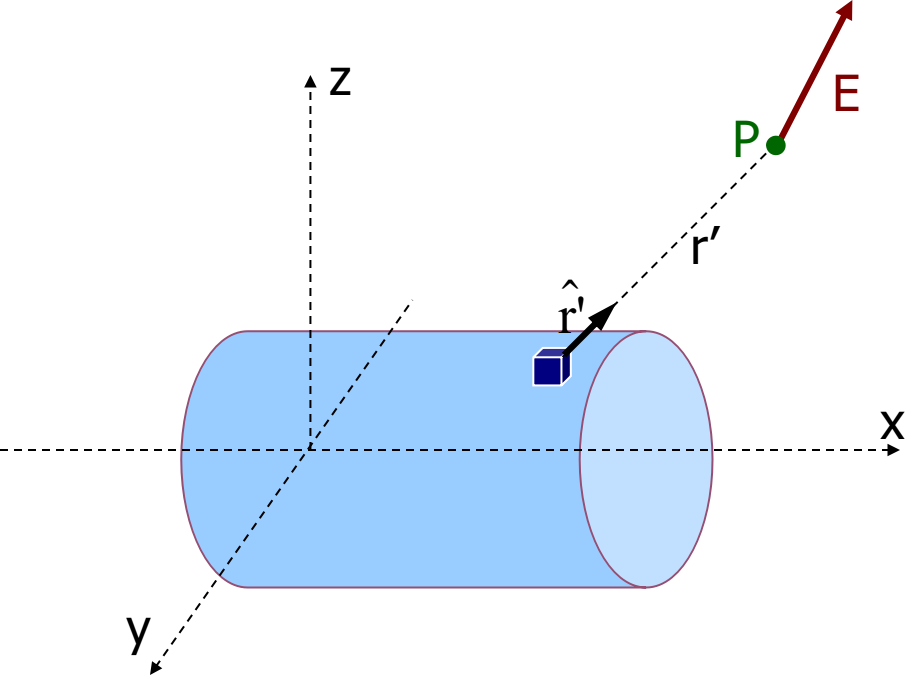
\includegraphics[width=200px]{6.png}
    \end{center}
    
    \[\vec E=k\int\limits_V \hat{r'} \frac{\rho(x,y,z) dV}{r'^2} \]

    Untuk densitas muatan pada bidang satu dimensi, dua dimensi dan tiga dimensi, \textbf{Jika distribusi muatan seragam, maka $\lambda, \sigma$ dan $\rho$ dapat diambil di luar integral} 

    \subsection{Densitas Muatan}%
    Ini semua hanya berlaku jika distribusi muatan seragam, maka $\lambda, \sigma$ dan $\rho$ dapat diambil di luar integral
    \begin{itemize}
        \item \textbf{Garis} Jika muatan terdistribusi pada sepanjang garis $\ell$, $\displayline \lambda \equiv \frac{Q}{\ell}$, satuannya adalah $C/m$.
        \item \textbf{Luas} Jika muatan terdistribusi pada luas permukaan A, maka $\displayline \sigma \equiv \frac{Q}{A}$, dengan satuan $C/m^2$
        \item \textbf{Volume} Jika muatan terdistribusi pada volume V, maka $\displayline \rho \equiv \frac{Q}{V}$ dengan satuan $C/m^3$
    \end{itemize}

    \subsection{Contoh Permasalahan Batang Bermuatan}%
    \textbf{Contoh 1:}\\
    Batang dengan panjang L memiliki muatan seragam per satuan panjang $\lambda$ dan $a$ muatan total $Q$. Hitung medan listrik pada titik P sepanjang sumbu batang pada jarak d dari salah satu ujungnya.

    \begin{center}
        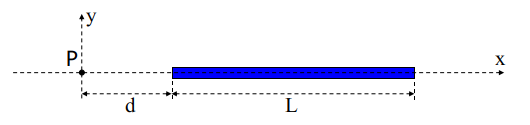
\includegraphics[width=220px]{7.png}
    \end{center}
    Mari kita letakkan asal di P. Kerapatan muatan linier dan $Q$ terkait dengan
        \[ \lambda=\frac{Q}{L}\ dan\ Q=\lambda L \]
    Kita anggap bahwa Q bermuatan Positif.

    \begin{center}
        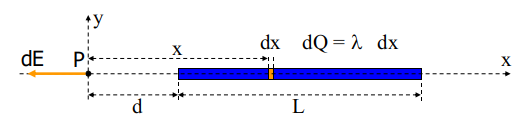
\includegraphics[width=220px]{8.png}
    \end{center}

    Titik medan listrik menjauh dari batang. Secara simetri, medan listrik pada sumbu batang tidak memiliki komponen $y$. $dE$ dari muatan pada panjang batang $dx$ yang sangat kecil adalah..

    \[ d \vec E=k\frac{dq}{x^2}=k\frac{\lambda\ dx}{x^2} \]

    Perlu diingat bahwa $d \vec E$ pada arah sumbu $-x$. $dE$ adalah harga/nilai dari vektor $d \vec E$. Kita gunakan fakta bahwa $Q>0$, maka $dq=0$ untuk menghilangkan tanda nilai absolut dalam persamaan awal.

    \begin{align*} 
        \vec E &= \int_d^{d+L} d\vec E_x\\
               &= -k \int_d^{d+L} \frac{\lambda dx}{x^2} \hat i\\
               &= -k \lambda \int_d^{d+L} \frac{dx}{x^2} \hat i\\
               &= -k \lambda \left( -\frac1x \right)_d^{d+L} \hat i\\
               &= -k \lambda \left( -\frac1{d+L} + \frac1d \right) \hat i\\
               &= -k \lambda \left(\frac{-d+d+L}{d(d+L)} \right) \hat i\\
               &= -k \frac{\lambda L}{d(d+L)} \hat i\\
               &= -\frac{kQ}{d(d+L)} \hat i
    \end{align*}

    \textbf{Contoh 2:}\\ 
    Sebuah batang dengan panjang $L$ memiliki muatan seragam per satuan panjang $\lambda$ dan muatan total $q$. Hitung medan listrik pada titik $P$ yang terletak pada jarak $a$ dari batang..
    \begin{center}
        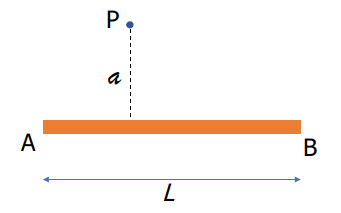
\includegraphics[width=140px]{9.png}
    \end{center}

    Pertama-tama, kita analisis persoalan tersebut dengan gambar analisis medan listrik
    \begin{center}
        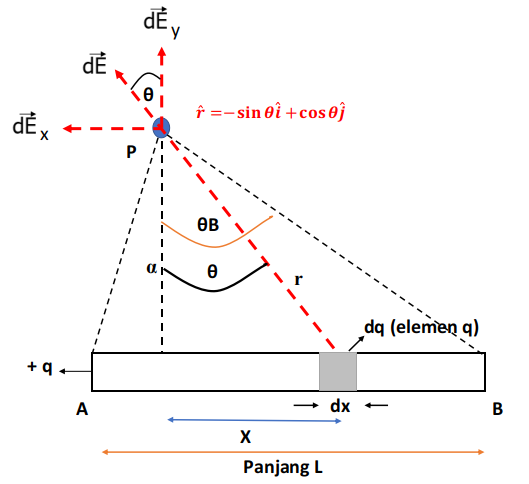
\includegraphics[width=220px]{10.png}
    \end{center}
    Kita ketahui bahwa kuat medan listrik di titik $P$ oleh batang $AB$ bermuatan $+Q$, maka
    \[ d\vec E = \frac1{4\pi \epsilon_0} \frac{dQ}{r^2} \hat r \]

    Rapat muatan per satuan panjang $\lambda$ pada kawat lurus homogen
    \[ \lambda = \frac{dQ}{dx} = \frac{q}L \]
    dimana $\frac{dQ}{dx}$ adalah densitas muatan per elemen yang dianggap sangat kecil dan $\frac{q}L$ adalah densitas muatan pada batang utuh, keduanya dianggap sama karena persebaran muatan pada sebuah batang dianggap homogen. Sehingga
    \[ dq =  \lambda\ dx \]
    Disamping itu, hubungan geometris antara $a$, $x$, dan $r$ adalah:
    \begin{align*}
        \cos \theta = \frac{a}r\ \rightarrow \frac1{r^2} &= \frac{\cos^2 \theta}{a^2}\\
        \tan \theta = \frac{x}a\ \rightarrow x&=a\ tan \theta\\
        dx &= a \frac1{cos^2 \theta} d\theta
    \end{align*}
    Maka
    \begin{align*}
        d \vec E &= k \frac{dQ}{r^2} \hat r= k \lambda \frac{dx}{r^2} \hat r^2\\       
        d \vec E &= k \lambda \frac{dx}{r^2} \hat r\\
        d \vec E &= k \lambda  (-\sin \theta \hat i + \cos \theta \hat j)\\
        d \vec E &= k \lambda  (dx \frac1{r^2} (-\sin \theta)\hat i + dx \frac1{r^2}(cos \theta) \hat j)\\
        d \vec E &= \frac{k \lambda}a (-\sin \theta d\theta \hat i +\cos \theta d\theta \hat j)\\
        \vec E &= \frac{k \lambda}a \int_{\theta A}^{\theta B} (-\sin \theta \hat i + \cos \theta \hat j)\\
        \vec E &= \frac{k \lambda}a [(\cos \theta_B - \cos \theta_A) \hat i + (\sin \theta_B - \sin \theta_A) \hat j ]
    \end{align*}

    Jika panjang kawat tak terhingga, maka \textbf{$\theta_B = 90 \degree$ dan $\theta_a=270 \degree$}, sehingga
    \[ \vec E = \frac{k \lambda}a 2 \hat j \]
    
    Pada sistem berikut ini, cara penurunan rumusnya sama, namun yang berbeda cuma $\hat r$ nya saja
    \begin{center}
        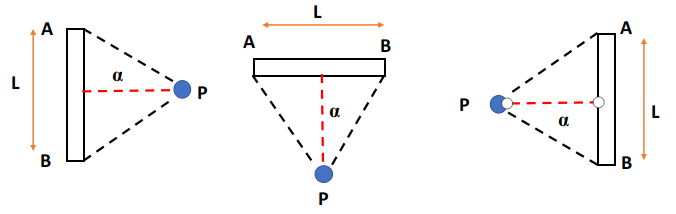
\includegraphics[width=220px]{11.png}
    \end{center}
    
    \subsection{Bagian cincin bermuatan listrik}%
    Akan dibahas bagaimana kuat medan listrik di pusat cincin P oleh bagian cincin AB
    \begin{center}
        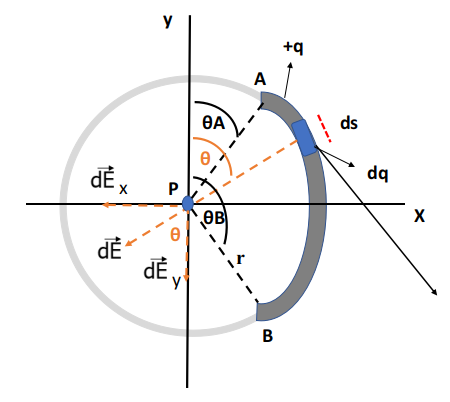
\includegraphics[width=180px]{12.png}
    \end{center}

    \[ d \vec E=\frac1{4\pi \epsilon_0} \frac{dq}{r^2}\hat r \]
    dengan $\hat r= -\sin \theta \hat i - \cos \theta \hat j$, maka
    \begin{align*}
        \lambda=\frac{dq}{ds}\ \rightarrow\ dq &= \lambda\ ds\\
        dq &= \lambda\ r\ d\theta
    \end{align*}

    \begin{center}
        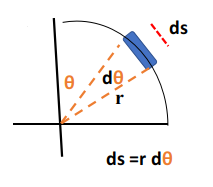
\includegraphics[width=100px]{13.png}
    \end{center}

    Sehingga,
    \begin{align*}
        d \vec E &= k \lambda \frac{dx}{r^2} \hat r\\
        d \vec E &= k \lambda \frac{rd \theta}{r^2} (-\sin \theta \hat i - \cos \theta \hat j)\\
        \vec E &= \frac{k \lambda}{r} \int_{\theta_A}^{\theta_B} (-\sin \theta \hat i - \cos \theta \hat j)\\
        \vec E &= \frac{k \lambda}{r} [(\cos \theta_B - \cos \theta_A)\hat i - (\sin \theta_B - \sin \theta_A)\hat j]
    \end{align*}

    Jika cincin penuh dan titik pengamatannya berada di tengah, maka yang terjadi adalah\\ $\theta_A\ =\ \theta_B\ \rightarrow$ saling meniadakan.

    \subsection{Sumbu Cincin Bermuatan Listrik}%
    Bagaimana kuat medan listrik pada titik P oleh cincin bermuatan?
    \begin{center}
        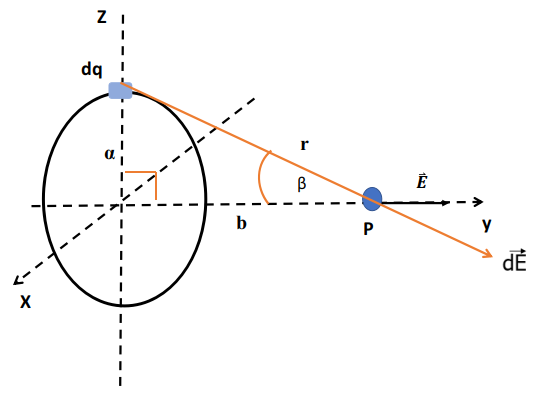
\includegraphics[width=220px]{14.png}
    \end{center}

    \[ d \vec E = \frac1{4\pi \epsilon_0} \frac{dq}{r^2} \hat r \]
    Dengan 
    \begin{align*}
        \hat r &= \cos a\hat i + \cos \beta \hat j + \cos \gamma \hat k\\
        \hat t &= \cos \beta \hat j
    \end{align*}
    Kenapa E total arahnya ke sumbu Y (hanya ada elemen di sumbu y)?? Jika ditinjau dari sumbu x dan sumbu z, cincin simetris dalam sumbu dan sumbu z, sehingga saling meniadakan. Maka
    \begin{align*}
        d \vec E&=\frac1{4\pi \epsilon_0}\frac{dq}{r^2} \hat r\\
        d \vec E&=\frac1{4\pi \epsilon_0}\frac{dq}{r^2} \cos \beta\hat j\\
        \vec E&=\frac{k\cos \beta\hat j}{r^2}\int dq\hat j\\
        \vec E&=\frac{k\ q}{r^2}\cos \beta \hat j\\
        \vec E&=\frac{k\ q}{(a^2+b^2)^{3/2}}\hat j\\
    \end{align*} 

    Dimana
    \[ q=\lambda \]
    \[ ds=\lambda\ 2\pi a \]
    \[ r^2=a^2+b^2\ \rightarrow\ cos \beta = \frac{b}r = \frac{b}{\sqrt{a^2+b^2}} \]

    \subsection{Medan Listrik di Bidang lingkaran/Disk/Cakram}%
    \begin{center}
        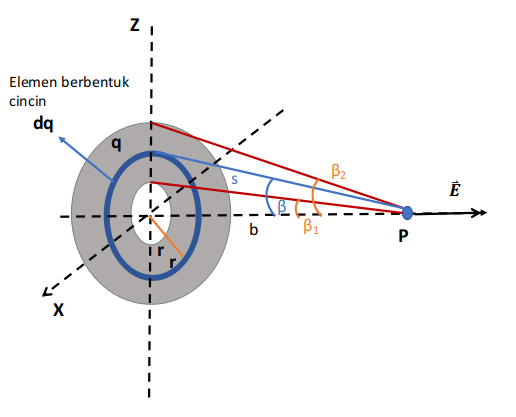
\includegraphics[width=220px]{15.png}
    \end{center}
    Rapat muatan persatuan luas adalah $\sigma$
    \[ \sigma=\frac{dq}{dA}= \frac{dq}{2\pi r\ dr}\ \rightarrow\ dq=\sigma2\pi r\ dr \]

    Medan listrik di titik P adalah
    \begin{align*}
        d\vec E &= \frac{k\ dq}{s^2} \cos \beta \hat j\\
        d\vec E &= \frac{k\ \sigma2\pi r\ dr}{s^2} \cos \beta \hat j\\
    \end{align*}
    dengan
    \begin{align*}
        \cos \beta=\frac{b}s\ \rightarrow\ \frac1{s^2}&=\frac{\cos^2\beta}{b^2}\\
        \tan \beta= \frac{r}b\ \rightarrow\ r&=b\ \tan \beta\\
        dr&= b\frac1{\cos^2\beta} d\beta
    \end{align*}

    Maka
    \begin{align*}
        \vec E&=k\sigma2\pi \int \frac{r\ dr}{s^2} \cos \beta \hat j\\
        \vec E&=k\sigma2\pi \int b \frac{\sin \beta}{\cos \beta} \frac{\cos^2 \beta}{b^2} b \frac1{\cos^2\beta}\ d\beta \cos \beta \hat j\\
        \vec E&=2\pi\sigma k \int_{\beta_1}^{\beta_2} \sin \beta\ d \beta \hat j\\
        \vec E&=2\pi\sigma k\ (-\cos \beta_2 + \cos \beta_1)\hat j\\
        \vec E&= \frac{\sigma}{2\epsilon_0} (-\cos\beta_2 + \cos\beta_1)\hat j
    \end{align*}
    Lalu jika bidang lingkaran penuh beradius\\ R $\rightarrow\ \beta_1=0$,
    Maka

    \begin{align*}
        \vec E&= \frac{\sigma}{2\epsilon_0} (-\cos\beta_2 + \cos0\degree)\hat j\\
        \vec E&= \frac{\sigma}{2\epsilon_0} (- \frac{b}{\sqrt{b^2+R^2}} + 1)\hat j\\
    \end{align*}
    Jika luas bidang lingkaran tak berhingga, maka $\beta_2 = 90\degree$ dan $\beta_1=0\degree$

    \begin{align*}
        \vec E&= \frac{\sigma}{2\epsilon_0} (-\cos90\degree + \cos0\degree)\hat j\\
        \vec E &= \frac{\sigma}{2\epsilon_0}
    \end{align*}

\end{document}
